
\documentclass[review]{elsarticle}
\usepackage{hyperref}
\usepackage[margin=1in]{geometry}
\usepackage{graphicx}
\usepackage{amsmath}
\usepackage{placeins}
\usepackage{comment}
\usepackage{fancyref}

\def\bibsection{\section*{References}}

\journal{Journal of Nuclear Materials}
\bibliographystyle{elsarticle-num}

\begin{document}
\begin{frontmatter}
\title{A modified Embedded-Atom Method interatomic potential for uranium-silicide}

\author[inl]{Benjamin Beeler\corref{qwe}}
\cortext[qwe]{Corresponding author}
\ead{benjamin.beeler@inl.gov}
\author[lanl,ucsd,msu]{Michael Baskes}
\author[lanl]{David Andersson}
\author[lanl]{Michael WD Cooper}
\author[inl]{Yongfeng Zhang}
\address[inl]{Idaho National Laboratory, Idaho Falls, ID 83415}
\address[lanl]{Los Alamos National Laboratory, Los Alamos, NM 87545}
\address[ucsd]{University of California-San Diego, San Diego, CA 92093}
\address[msu]{Mississippi State University, MS 39762}


\begin{abstract}

Uranium-silicide (U-Si) fuels are being pursued as a possible accident tolerant fuel (ATF).  This uranium alloy fuel benefits from higher thermal conductivity and higher fissile density compared to uranium dioxide (UO$_{2}$).  In order to perform engineering scale nuclear fuel performance simulations, the material properties of the fuel must be known.  Currently, the experimental data available for U-Si fuels is rather limited.  Thus, multiscale modeling efforts are underway to address this gap in knowledge.  In this study, a semi-empirical modified Embedded-Atom Method (MEAM) potential is presented for the description of the U-Si system.  The potential is fitted to the formation energy, defect energies and structural properties of U$_{3}$Si$_{2}$. The primary phase of interest (U$_{3}$Si$_{2}$) is accurately described over a wide temperature range and displays good behavior under irradiation and with free surfaces.  The potential can also describe a variety of U-Si phases across the composition spectrum.  

\end{abstract}
\end{frontmatter}

\section{Introduction}

Nuclear fuels operate in reactor environments experiencing high temperatures, temperature gradients and mechanical stress under irradiation.  This complex and extreme environment, combined with the high power density that allows nuclear fuels to be economical, presents safety challenges during off-normal events and accidents.  In addition to innovations in reactor design, research is focused on the development of advanced materials \cite{zinkle2016} to improve accident tolerance.  Accident-tolerant fuel (ATF) \cite{zinkle2014} is being considered as a potential fuel for future and existing light-water reactors (LWRs).  ATFs aim to provide additional coping time in the event of an accident (such as a loss of coolant accident) due to the inherent properties of the fuel, while maintaining good operational characteristics.  Uranium-silicide (U-Si), and particularly U$_{3}$Si$_{2}$, is being considered as a fuel candidate for ATFs.  U$_{3}$Si$_{2}$ exhibits higher uranium density than traditional UO$_{2}$ LWR fuel, thus allowing for the possibility of reduced enrichments, fewer assemblies and/or an extended lifetime in the core.  U$_{3}$Si$_{2}$ also possesses a higher thermal conductivity than UO$_{2}$, allowing for a lower fuel centerline temperature and more rapid heat removal during off-normal conditions.  

In order for the implementation of U$_{3}$Si$_{2}$ to become a reality, the scientific community should be able to perform continuum scale descriptive and predictive nuclear fuel performance simulations.  To perform such simulations, the material properties of the fuel must be known.  Subjecting U$_{3}$Si$_{2}$ to the in-reactor environment leads to microstructural changes due to the evolution of radiation produced defects, segregation and precipitation of fission products, and mechanical deformation. These changes in fuel microstructure change fuel properties, directly impacting fuel performance and safety.  The ability to understand and model microstructural changes throughout the lifetime of the fuel is critical in developing fuel performance modeling codes.  The current experimental data available for U-Si fuels is incomplete, but does include crystal structures \cite{zachariasen1949, remschnig1992}, phase diagrams \cite{massalski1990}, thermal conductivity, heat capacity, thermal expansion \cite{white2015, shimizu1965}, high pressure diffraction \cite{yagoubi2013}, formation enthalpies \cite{gross1962, ohare1975, alcock1962, rand1963, berche2009} and irradiation studies \cite{shimizu1965, finlay2002}.  Information that has not yet been investigated via experimentation includes elastic properties, diffusion coefficients, displacement energy, variation of thermal conductivity with porosity, fission product properties within various USi phases and interfacial properties, to name a few.  Thus, multiscale modeling efforts are underway to address this gap in knowledge.

One recent investigation involved first principles calculations characterizing a variety of properties in the U-Si system \cite{noordhoek2016}.  These calculations have been able to provide insight where experimental information is lacking.  However, first principles calculations are limited in their ability to investigate systems larger than a few hundred atoms in size, and are severely restricted in their ability to investigate properties at non-zero temperatures.  Thus, although these types of investigations are of critical importance, branching to higher time and length scales is necessary for the investigation of larger, more complex systems.  Molecular dynamics-density functional theory (MD-DFT) can be employed to look at non-zero temperatures, but are still restricted to a very small system size and very short time scale.  In order to overcome this limitation, interatomic potentials can be employed within molecular dynamics (MD) methods to solve Newton's equations of motion.  In this way, MD can be used to calculate relevant properties above 0 K on a nanosecond time and nanometer spatial scale.  Information obtained from molecular statics and dynamics simulations can then be input into higher level modeling methodologies such as phase field, kinetic Monte Carlo or continuum level finite element modeling.  In this manner, physics-based multiscale microstructural evolution models can be generated.  Thus, development of an interatomic potential to describe the U-Si system is a critical step in branching time and length scales with the long-term goal of developing a descriptive and predictive nuclear fuel performance code.

Very few interatomic potentials have been constructed for uranium-based alloys.  This is due to the inherent difficulty in describing the behavior of f-electrons and the mechanical instability of the $\gamma$ phase of uranium at low temperatures.   Several interatomic potentials have been developed for pure uranium \cite{beeler_meam, beelerASTM, fernandez2014, li2011, smirnova2012, li2012}, with only a few being adapted into alloy potentials for U-Zr \cite{moore2015},  U-Al \cite{pascuet2012} and U-Mo \cite{smirnovaUMo}.  Based on the functionality of the modified Embedded-Atom Method (MEAM) variants of U and U-Zr \cite{beeler_meam, moore2015} as well as their inclusion of fission gases Xe, Kr and He \cite{beelerASTM}, it is determined that this is a suitable potential form to pursue in attempting to describe the U-Si system.  

This manuscript presents a MEAM interatomic potential for the description of the U-Si system, with particular emphasis on U$_{3}$Si$_{2}$.  No interatomic potentials for the U-Si system have been constructed prior to this work.

 
\section{MEAM Theory}
The Embedded-Atom Method (EAM) \cite{daw1984, daw1993, daw1983} has been shown to predict the properties of alloys and metals quite well. The EAM is the most widely used semi-empirical potential, with applications including calculations of point defects \cite{olsson2009}, melting \cite{belaschenko2011}, grain boundary structure and energy \cite{liu1999}, dislocations \cite{chassange2011} [40], segregation \cite{li2009MatChem}, fracture \cite{vatne2011} and surface structure \cite{rose1984}.  The basis of the EAM is that the cohesive energy can be expressed in terms of embedding energies.  In this view, each atom in the metal is embedded into the electron gas created by the other atoms.  The EAM provides a robust means of calculating structure and energetics; however, it is best suited strictly for purely metallic systems with no directional bonding.
From the EAM, the total energy of a system of atoms is given by equation \ref{eq:eqn1}:


\begin{equation}
\label{eq:eqn1}
E = \sum_{i} \{F(\bar{\rho}_{i})\ +  \frac{1}{2} \sum_{j \neq i} S_{ij}\phi(R_{ij})   \}
\end{equation}

where $i$ and $j$ are the individual atoms of the model \cite{daw1983, daw1984}.  The pair interaction between atoms $i$ and $j$ is given by $\phi$ \cite{baskes1992} and is dependent on the separation between the atoms $R_{ij}$.

\begin{equation}
\label{eq:eqn2}
\phi(R) = \frac{2}{Z} \Bigl\{ E^{u}(R) - F( \frac{ \bar{ \rho}^{0}(R)}{Z}) \Bigr\}  
\end{equation}

In equation \ref{eq:eqn2}, $Z$ is the number of first neighbors, $\bar{ \rho}^{0}(R)$ is the background electron density and $\{E^{u}(R)$ is the per atom energy of the reference structure as a function of nearest-neighbor distance $R$ \cite{baskes2000} obtained from the universal equation of state of Rose et al. \cite{rose1984} given in equation \ref{eq:eqn3}.

\begin{equation}
\label{eq:eqn3}
 E^{u}(R) = -E_{c} (1 + a^{*} + \delta \times (\frac{r_{e}}{r}) \times (a^{*})^{3}) e^{(-a^{*})}
 \end{equation}

with

\begin{equation}
\label{eq:eqn4}
a^{*} = \alpha ( \frac{R}{r_{e}} - 1)
\end{equation}

and

\begin{equation}
\label{eq:eqn5}
\alpha^{2} = \frac{9\omega B}{E_{c}}
\end{equation}

where E$_{c}$, r$_{e}$, $\omega$ and B are the cohesive energy, nearest neighbor distance, atomic volume and bulk modulus, respectively, evaluated at equilibrium in the reference structure.  The background electron density is given by:

\begin{equation}
\label{eq:eqn6}
\bar{\rho}^{0}(R) = Z \rho^{a(0)} (R)
\end{equation}

where $\rho^{a(0)}$  is an atomic electron density discussed below.  The embedding function, F, is given in equation \ref{eq:eqn7} and is the energy required to embed atom i into a system with a background electron density $\bar{\rho}_{i}$.  

\begin{equation}
\label{eq:eqn7}
F(\bar{\rho}) = AE_{c} \frac{\bar{\rho}}{Z}\ln\frac{\bar{\rho}}{Z}
\end{equation}

The modification to the EAM is a function of how the electron density at a certain point, $\rho_{i}$, is calculated.  In the traditional EAM, $\rho_{i}$ is simply the linear supposition of spherically averaged atomic electron densities:

\begin{equation}
\label{eq:eqn8}
\rho_{i}^{(0)} = \sum_{j \neq i} \rho_{j}^{a(0)} (R_{ij})
\end{equation}

whereas the MEAM introduces angularly dependent terms to augment $\bar{\rho_{i}}$ as shown in equation \ref{eq:eqn9} through equation \ref{eq:eqn11} \cite{baskes2000, baskes1987}.  

\begin{equation}
\label{eq:eqn9}
(\rho_{i}^{(1)})^{2}=\sum_{\alpha} \{ \sum_{j \neq i}x_{ij}^{\alpha}\rho_{i}^{a(1)}(R_{ij})\}^{2} = \sum_{j,k \neq i}\rho_{j}^{a(1)}(R_{ij})\rho_{k}^{a(1)}(R_{ik})cos\{\theta_{ijk}\}
\end{equation}

\begin{equation}
\label{eq:eqn10}
(\rho_{i}^{(2)})^{2}=\sum_{\alpha,\beta}\{\sum_{j \neq i}x_{ij}^{\alpha}x_{ij}^{\beta}\rho_{j}^{a(2)}(R_{ij})\}^{2} - \frac{1}{3}\sum_{j \neq i}[\rho_{j}^{a(2)}(R_{ij})]^2
\end{equation}

\begin{equation}
\label{eq:eqn11}
(\rho_{i}^{(3)})^{2}=\sum_{\alpha,\beta,\gamma}\{ \sum_{j \neq i}x_{ij}^{\alpha}x_{ij}^{\beta}x_{ij}^{\gamma}\rho_{j}^{a(3)}(R_{ij}) \}^{2} - \frac{3}{5}\sum_{j \neq i}[\rho_{j}^{a(3)}(R_{ij})]^2
\end{equation}

Here, the $\rho^{a(l)}$  are the atomic densities which represent the decrease in the contribution with distance R$_{ij}$ and the $\alpha$, $\beta$, $\gamma$ summations are each over the three coordinate directions with x$_{ij}^{\alpha}$ being the distance the ratio R$_{ij}^{\alpha}$/R$_{ij}$ with R$_{ij}^{\alpha}$ being the $\alpha$ component of the distance vector between atoms i and j [29].  Similar to equation \ref{eq:eqn9}, equations \ref{eq:eqn10} and \ref{eq:eqn11} can be put in a form that has a dependence on the angle between atoms i, j and k ($\theta_{ijk}$), and this has been done by Baskes et al. \cite{baskes1989}.  Atomic electron densities are assumed to decrease exponentially, 

\begin{equation}
\label{eq:eqn12}
\rho_{i}^{a(l)}(R) = e^{[-\beta^{(l)}(\frac{R}{r_{e}}-1)]}
\end{equation}

where $\beta^{(l)}$ are the decay constants.  To obtain the background electron density from the partial electron densities we make the assumption that the angular terms are a small correction to the EAM.

\begin{equation}
\label{eq:eqn13}
\bar{\rho}^{2} = \sum_{l=0}^{3}\bar{t}_{i}^{(l)} (\rho_{i}^{(l)})^{2}
\end{equation}

where the $\bar{t}_{i}^{(l)}$ \cite{valone2006} are combinations of model constants $t^{l}$ that are associated with the atom types of neighbors $i$.

Many body screening is implemented through a screening function, S$_{ij}$, that quantifies screening between two atoms i and j due to other atoms in the system, k.  The atomic electron densities and the pair potential are multiplied by this function.  The screening function depends on all other atoms in the system:

\begin{equation}
\label{eq:eqn14}
S_{ij}=\Pi_{k \neq i,j}S_{ijk}
\end{equation}

where S$_{ijk}$ is calculated using a simple geometric construction.  The screening factor S$_{ijk}$ is defined as:

\begin{equation}
\label{eq:eqn15}
S_{ijk}= f_{c}\left[\frac{C-C_{min}}{C_{max}-C_{min}}\right]
\end{equation}

where C is a geometric parameter, and C$_{min}$ and C$_{max}$ are limiting values of C.  The smooth cutoff function is:

\begin{equation}
\label{eq:eqn16}
f_{c}(x) = \begin{cases}
    1       & \quad x \geq 1 \\
    [1-(1-x)^{6}]^{2}  & \quad 0 < x < 1\\
    0       & \quad x \leq 0\\
  \end{cases} 
\end{equation}

A radial cutoff function is also applied to the atomic electron densities and pair potential which is given by f$_{c}[(r_{c}-r)/\lambda]$ where r$_{c}$ is the cutoff distance of 6 {\AA } and $\lambda$ gives the cutoff region and was chosen to be 0.1 {\AA}.  The MEAM has been shown to accurately predict the behavior of complex systems such as plutonium \cite{baskes2000} and tin \cite{baskes1997}.  It should be noted that these equations are for a single component system and can be generalized for a multicomponent system, as was done in \cite{baskes2014}.  

\section{Fitting Procedure}
In order to create a functional uranium-silicide (U-Si) binary interatomic potential, there must first exist (or be generated) suitable potentials for each individual element.  A uranium potential from Moore, $\textit{et al.}$ \cite{moore2015} is utilized in the fitting.  This MEAM interatomic potential performs excellently in describing the body-centered cubic phase of uranium and the alloy behavior of UZr.   

For the Si MEAM contribution, the initial potential utilized was from Baskes \cite{baskes1992}.  Upon finding this potential over-predicted the Si-Si dimer distance (compared to the reference value of 2.25 \AA \cite{huber1979}), underestimated the melting point and overestimated the thermal expansion, the fitting of a new Si-Si potential was undertaken in an attempt to rectify these discrepancies.  Allowing all MEAM parameters to vary, the Si MEAM potential was fit to targets of the elastic constants, vacancy formation energy, thermal expansion, a theoretical face-centered cubic structure, a Si-Si dimer and a quenched melted structure.  This modified Si MEAM potential increased the melting point, slightly decreased the dimer distance and decreased the thermal expansion without significant degradation of 0 K pure diamond cubic Si properties.  This potential was then utilized in the development of a U-Si MEAM binary potential.  

The fitting procedure to develop cross-species parameters (U-Si interactions) involves a reference phase (L1$_{2}$-U$_{3}$Si), a starting guess for MEAM parameters, and is then refined via a script that gives a random step to all relevant MEAM parameters.  This updated potential is then input into LAMMPS \cite{plimpton1995} and a series of simulations are performed, the output of which is utilized to calculate a weighted-error summation.  The script then either accepts or rejects the prescribed changes to the MEAM parameters based on the reduction of the total weighted-error.  The emphasis of the fitting procedure was the U$_{3}$Si$_{2}$ phase, which possesses a relatively complex crystal structure, with a 10 atom unit cell in space group P4/$\textit{mbm}$-No. 127, two unique uranium atomic sites (2a (0, 0, 0) and 4h (0.181, 0.681, 0.5) ) and one unique silicon atomic site (4g (0.389, 0.889, 0) ), as first reported by Zachariasen \cite{zachariasen1949}.  The cohesive energy, lattice constants and elastic constants of the U$_{3}$Si$_{2}$ phase were given priority with respect to the error weighting, and are thus considered the primary fitting targets.  Additionally, a number of alternative structures were discovered throughout the fitting procedure via a heating and quenching simulation.  Up to eight alternative structures were included as fitting targets at a given time, enforcing the condition that these structures exhibited a higher energy than the experimental structure.  A variety of other simulations were performed periodically to serve as sanity checks for the potential, examples of which include a heating and cooling stage, inclusion of defects and investigation of other U-Si theoretical phases, but these were not included as fitting targets.  In this primary fitting stage, only cross-species parameters were allowed to vary.  

Upon completion of the primary fitting stage, a full examination of the potential's strengths and weaknesses was performed, investigating not only the accuracy of the fitting targets, but the ability of the potential to predict the defect properties of U$_{3}$Si$_{2}$, the relative formation energy of a variety of other U-Si phases and the melting point of U$_{3}$Si$_{2}$.  A secondary fitting stage was then undertaken that included select dilute defect formation energies as fitting targets, in addition to the targets in the primary fitting stage.  In this secondary stage, the variation of MEAM parameters was not restricted to only U-Si cross species parameters, but all pure Si MEAM parameters were also given the freedom to change.  This modification was motivated by the lack of importance in accurately predicting pure Si properties, especially in a system that is U-rich, as low Si content phases will not exist in these nuclear fuel systems.  In this way, the potential was fine tuned to more accurately reflect defect properties, while retaining accuracy in predicting the energetics and elastic properties of U$_{3}$Si$_{2}$.  

The final Si MEAM potential is shown in Table \ref{tab:ben2} alongside the U MEAM potential for clarity.  The U-Si MEAM cross-species potential parameters are shown in Table \ref{tab:ben3}.  Screening parameters are given in LAMMPS format (i.e., C$_{max}$(I,J,K) is a screening parameter when I-J pair is screened by K, where I, J and K are atom types).  Readers can refer to the LAMMPS \cite{plimpton1995} documentation for full implementation of these parameters.  

\begin{table}[h]
\caption{Silicon and Uranium MEAM potential parameters}\label{tab:ben2}
\begin{center}
\begin{tabular}{|c|c|c|}
     \hline
     Parameter & Si-MEAM  & U-MEAM  \\
     \hline
     attrac & -0.2073 & 0.105  \\
     repuls & -0.1876 & 0.105 \\
     alpha & 5.5576 & 5.5   \\
     $\beta$$^{0}$ & 4.0501 & 4.8  \\
     $\beta$$^{1}$ & 5.6911 & 6  \\
     $\beta$$^{2}$ & 4.5856 & 6 \\  
     $\beta$$^{3}$ & 5.5305 & 6  \\
     alat (\AA) & 5.431 & 4.28  \\
     E$_{c}$ (eV) & 4.63 & 5.27 \\
     A & 0.829 & 0.98 \\
     t$^{0}$ & 1 & 1 \\
     t$^{1}$ & 2.0601 & 2.5  \\
     t$^{2}$ & 4.6769 & 4.0 \\
     t$^{3}$ & -1.3216 & 1.2  \\
     C$_{min}$ & 0.9666 & 1.0 \\ 
     C$_{max}$ & 2.7994 & 1.9  \\
     \hline
\end{tabular}
\end{center}
\label{default}
\end{table}%


\begin{table}[h]
\caption{Uranium-silicon MEAM potential parameters.  Uranium is atom type 1 and silicon is atom type 2.}\label{tab:ben3}
\begin{center}
\begin{tabular}{|c|c|}
     \hline
     Parameter & U-Si MEAM \\
     \hline
     E$_{c}$ (eV) & 5.36 \\ 
     r$_{e}$ (\AA) & 3.05 \\
     lattce & l12 \\
     r$_{c}$ (\AA) & 6.0 \\
     attrac & -0.1129  \\
     repuls & 0.2171  \\
     alpha(1,2) & 4.793  \\
     rho(2) & 1.0727 \\
     rho(1) & 1 \\
     C$_{min}$(1,1,2) & 0.985 \\
     C$_{max}$(1,1,2) & 2.313 \\
     C$_{min}$(1,2,1) & 0.385 \\
     C$_{max}$(1,2,1) & 1.974 \\
     C$_{min}$(1,2,2) & 0.926 \\
     C$_{max}$(1,2,2) & 2.718 \\
     C$_{min}$(2,2,1) & 1.175 \\  
     C$_{max}$(2,2,1) & 1.435 \\
     \hline
\end{tabular}
\end{center}
\label{default}
\end{table}%

For the sake of clarity and reproducibility, LAMMPS MEAM-specific parameters are included in Table \ref{tab:ben4}.  It should also be noted that a non-standard implementation of MEAM within LAMMPS (which relates to modification of the smooth cutoff function) was utilized for the existing U MEAM potential and the subsequent U-Si potentials.  Please contact the authors to obtain the required modifications in order to accurately utilize the potential.  

\begin{table}[h!]
\caption{LAMMPS MEAM-specific parameters \cite{plimpton1995}.}\label{tab:ben4}
\begin{center}
\begin{tabular}{|c|c|}
     \hline
     Parameter & U-Si MEAM  \\
     \hline
     bkgd\_dyn & 1 \\
     nn2 & 1 \\
     delr (\AA)& 0.1 \\
     ialloy & 1 \\
     augt1 & 0 \\
     emb\_lin\_neg & 1 \\
     \hline
\end{tabular}
\end{center}
\label{default}
\end{table}%

\clearpage

\section{U-Si MEAM Potential Results}

The results for fundamental properties of U$_{3}$Si$_{2}$ at 0 K are displayed in Table \ref{tab:ben5} and compared to experiments \cite{zachariasen1949, berche2009} and DFT calculations \cite{noordhoek2016} (DFT+U results from \cite{noordhoek2016} are used for comparison but are simply referred to as DFT here).  For the U-Si MEAM potential, the formation energy is very accurate while the volume per atom is slightly underestimated.  The $\it{a}$ lattice constant is underestimated and the $\it{c}$ lattice constant is slightly overestimated.  The elastic constants show varying degrees of agreement with DFT predictions.  Excellent agreement is shown for G$^{xz}$ (equation \ref{eq:gxz}), C$_{33}$ and C$_{66}$, but significant variance is observed for C$_{12}$, for example.  The resulting bulk modulus, calculated via the elastic constants in equation \ref{eq:bulk}, is overestimated.  The bulk modulus was also calculated via the Birch-Murnaghan curve \cite{cohen85, birch47}, yielding a value of 134.5 GPa, which is consistent with the calculation of the bulk modulus via elastic constants.  There is observed a general over-stiffness prediction of the elastic constants.  The root-mean-square error over the nine calculated elastic constants is 55.0 GPa.  

\begin{equation}
\label{eq:gxy}
G^{xy}= \frac{\frac{C_{11} + C_{22}}{2} - C_{12}}{2}
\end{equation}

\begin{equation}
\label{eq:gxz}
G^{xz}= \frac{\frac{C_{11} + C_{33}}{2} - C_{13}}{2}
\end{equation}

\begin{equation}
\label{eq:bulk}
B=(C_{11} + C_{22} + C_{33} + 2*C_{12} + 2*C_{13} + 2*C_{23})/9
\end{equation}

\begin{table}[h!]
\caption{Properties of U$_{3}$Si$_{2}$ at 0 K.  Results from the MEAM U-Si potential are compared to experiments$^{1}$\cite{zachariasen1949}$^{2}$\cite{berche2009} and DFT$^{3}$\cite{noordhoek2016} calculations.  Units are as follows: E (eV/atom), V/at (\AA$^{3}$/atom), a and c (\AA), C$_{xx}$, B and G (GPa). }\label{tab:ben5}
\begin{center}
\begin{tabular}{|c|c|c|}
     \hline
      & Reference & U-Si MEAM  \\
     \hline
     E & -0.356$^{2}$ & -0.335 \\
     V/at & 20.844$^{1}$ & 20.355 \\
     a & 7.32$^{1}$ & 7.078 \\
     c & 3.89$^{1}$ & 4.063 \\
     c/a & 0.531$^{1}$ & 0.574 \\
     C$_{11}$ & 149$^{3}$ & 210.2  \\
     C$_{33}$ & 139$^{3}$ & 160.2 \\
     C$_{12}$ & 49$^{3}$ & 178.9 \\
     C$_{13}$ & 48$^{3}$ & 65.8 \\
     C$_{44}$ & 63$^{3}$ & 103.1 \\
     C$_{66}$ & 46$^{3}$ & 35.4 \\
     B & 81$^{3}$ & 134 \\
     G$^{xy}$ & 50$^{3}$ & 16  \\
     G$^{xz}$ & 48$^{3}$ & 60 \\
     \hline
\end{tabular}
\end{center}
\label{default}
\end{table}%

\FloatBarrier

The U$_{3}$Si$_{2}$ structure is shown in Figure \ref{fig:ben1} \cite{zachariasen1949}.  This figure illustrates a supercell of 2$\times$2$\times$3 unit cells with periodic boundaries.  In comparing the experimental structure to the predicted structures from the MEAM potential, minute differences are observed.  There is a slight expansion of uranium atoms (red) in the purely uranium plane and a minuscule clockwise rotation of atoms in the unit cell, with respect to the experimental structure.  This alteration is nearly imperceptible, except by analyzing the radial distribution function (RDF), as shown in Figure \ref{fig:benrdf}.  The RDF shows that the predicted structure from the MEAM potential is not capturing the smallest interatomic distance; this is due to the slight expansion in the U plane and the clockwise rotation of U and Si atoms.  These minor distortions slightly increase the first nearest neighbor distance (Si-Si) by approximately 0.2 {\AA} and slightly decrease the second and third nearest neighbor distances, as shown in Figure \ref{fig:benrdf} in the distance regime of 2.8-3 {\AA}.  
\begin{comment}
The first nearest-neighbor distance is a Si-Si distance.  It is possible this is overestimated due to the inherent properties of the Si MEAM potential, which slightly over-predicts the Si-Si dimer distance.  
\end{comment}
\begin{figure}[ht]
	\centering
	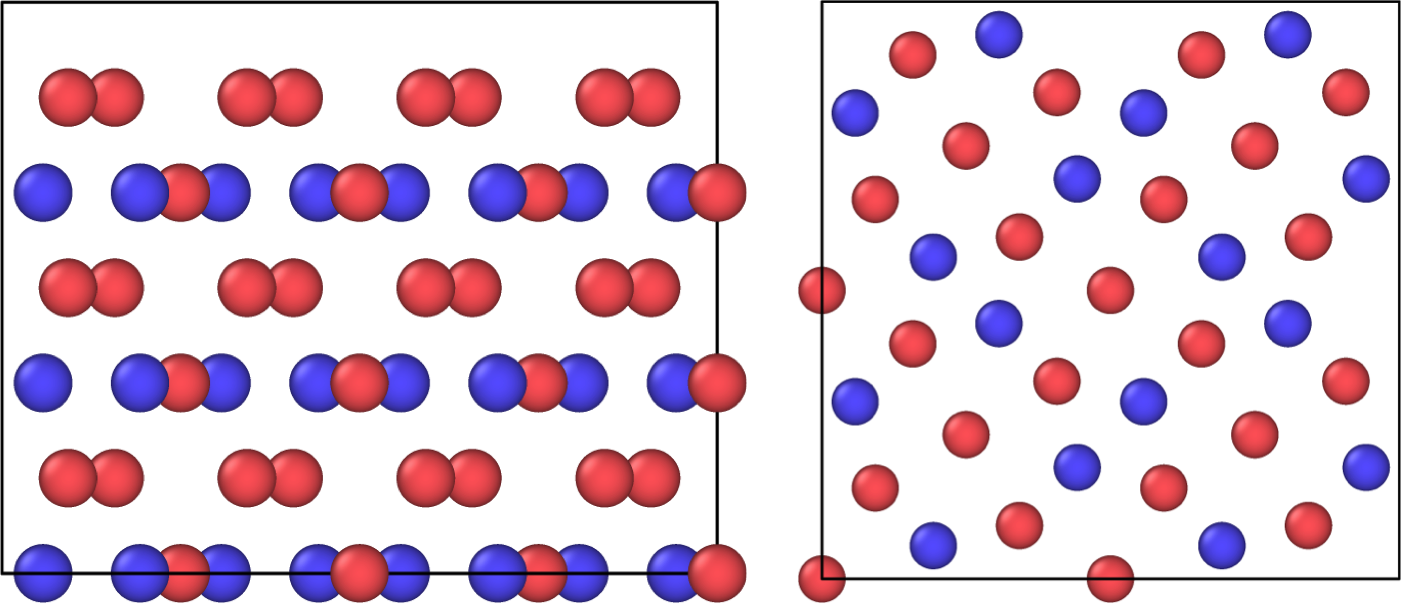
\includegraphics[width=0.8\textwidth]{ben1NEW.png}
    \caption{(100) view (left) and (001) view (right) of the experimental structure of U$_{3}$Si$_{2}$.  Uranium atoms in red; silicon atoms in blue.}\label{fig:ben1}
\end{figure}  

\begin{figure}[ht]
	\centering
	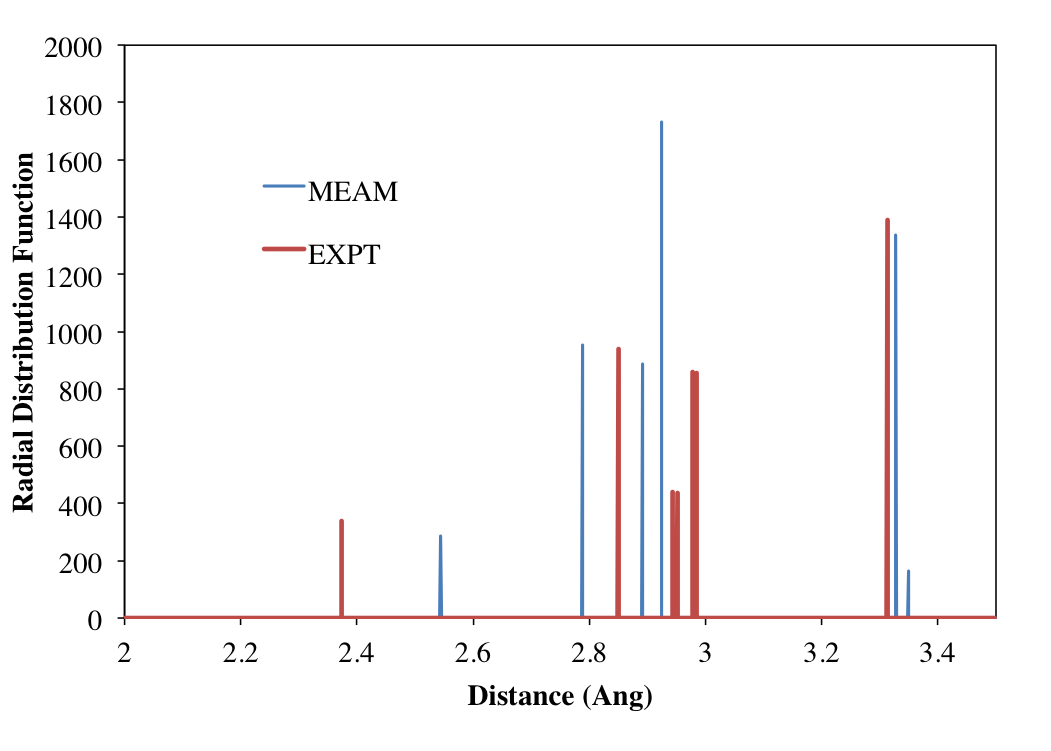
\includegraphics[width=0.8\textwidth]{rdfKK1.png}
    \caption{Radial distribution functions of U$_{3}$Si$_{2}$, comparing the MEAM predicted structures with the experimental structure.}\label{fig:benrdf}
\end{figure}

\FloatBarrier

Moving beyond the perfect crystal, the next step in testing the accuracy of the potential is to investigate point defects.  Single point defects (vacancy, interstitial, anti-site) were considered as a means of accommodating a change in stoichiometry.  The methodology for calculating point defect energetics is outlined in \cite{middleburgh2016}.  Point defect energies at 0 K for the U$_{3}$Si$_{2}$ system are shown in Table \ref{tab:ben6} and compared to results from DFT \cite{middleburgh2016}.  Bound Schottky defects are also shown in Table \ref{tab:ben6}.  There are two unique uranium sites in the U$_{3}$Si$_{2}$ structure.  Both U sites are investigated and denoted simply as U1 (for the 2a site) or U2 (for the 4h site), as in Remschnig, $\textit{et al.}$ \cite{remschnig1992}.  The lowest energy interstitial site is determined via a molecular dynamics simulation performed at 1000 K that was then quenched down to 0 K and subsequently minimized.   In this way, the interstitial is able to reorient itself into the most preferable configuration.  Three unique simulations were performed to ensure the lowest energy configuration was obtained.  The bound Schottky defect consists of two U2 vacancies, one U1 vacancy and two Si vacancies, such that crystallographic and stoichiometric accuracy is maintained.  Excellent agreement is observed for the formation energy of the U2 vacancy, Si vacancy, U interstitial, Si interstitial and the U1 antisite.  Reasonable agreement is observed for the U2 anti-site defect.  The U1 vacancy and Si antisite formation energies are overestimated.  The overestimation of the U1 vacancy likely leads to the slight overestimation of the bound Schottky defect formation energy.  

\begin{table}[h!]
\caption{Properties of point defects in U$_{3}$Si$_{2}$ at 0 K.  Results from the MEAM U-Si potential are compared to DFT calculations \cite{middleburgh2016}.  Units in eV.}\label{tab:ben6}
\begin{center}
\begin{tabular}{|c|c|c|}
     \hline
      &  DFT & U-Si MEAM \\
     \hline
     U1 vac & 0.68 & 1.16 \\
     U2 vac & 1.20 & 1.25 \\
     Si vac & 1.59 & 1.70 \\
     U int & 0.76 & 0.71 \\
     Si int & 0.19 & 0.28 \\
     U1 anti & 0.16 & 0.23 \\
     U2 anti & 0.35 & 0.60 \\
     Si anti & 0.35 & 1.17 \\
     Schottky Bound & 7.57 & 9.58  \\
     \hline
\end{tabular}
\end{center}
\label{default}
\end{table}%

In order to ensure that the potentials are not restricted to studying only the U$_{3}$Si$_{2}$ phase, other phases, experimental and theoretical, were examined that were not included in the fitting procedure.  These include the FeB-USi, B1-USi, AlB$_{2}$-USi$_{2}$, L1$_{2}$-USi$_{3}$, U$_{3}$Si$_{5}$ phases and the L1$_{2}$, $\alpha$ and $\beta$ phases of U$_{3}$Si.  The results are shown in Figure \ref{fig:eform3}  for the energy per atom and in Figure \ref{fig:vol3} for the volume per atom across the composition range.  In Figure \ref{fig:eform3}, excellent agreement is observed for the U-rich portion of the composition range.  For U$_{3}$Si and U$_{3}$Si$_{2}$, formation energies are nearly identical to those from experiments \cite{berche2009} and DFT calculations \cite{noordhoek2016}.  The lowest energy structure is the U$_{3}$Si$_{2}$ phase, which is the phase of primary interest, however this does not match the experimental or DFT results, which find the USi$_{2}$ and U$_{3}$Si$_{5}$ (a distorted USi$_{2}$ structure with $\frac{1}{6}$ of the silicon sites vacant) structures to be lowest in energy, respectively.  The MEAM potential correctly predicts the FeB-USi phase to be lower in energy than the B1-USi phase, but overestimates the formation energy of FeB-USi.  Significant variance is observed for the USi$_{3}$ structure.  Generally, there does exist a convex hull shape to the formation energy versus composition curve, which agrees with experiments \cite{berche2009} and DFT.  

In Figure \ref{fig:vol3}, there is a general negative parabolic trend in the volume predicted as a function of composition, which matches the trends from DFT and experiments quite well.  The volume per atom is slightly overestimated in the Si-rich portion of the composition range.  Per-atom volumes of USi, U$_{3}$Si$_{2}$ and U$_{3}$Si agree very well.  Given that only U$_{3}$Si$_{2}$ was utilized as a fitting target and L1$_{2}$-U$_{3}$Si was utilized as a reference structure, there is considerable agreement across the entire composition spectrum when comparing MEAM predicted results to the results from DFT calculations.   

It should be noted that DFT (GGA without Hubbard U) calculations \cite{noordhoek2016} found the presence of another structure for U$_{3}$Si$_{2}$ that is lower in energy than the experimental structure.  This structure was destabilized by the addition of the Hubbard U term, which resulted in the correct prediction of the experimental structure as the ground state.  In order to ensure no such low energy structure exists in the MEAM potential energy landscape, this alternate U$_{3}$Si$_{2}$ structure was analyzed.  In order to ensure all possible transformations and relaxations were allowed, a molecular dynamics simulation was performed at 500 K, followed by a quench to 0 K and a subsequent minimization.  Throughout the entire relaxation process, each of the six components of the stress tensor are independently controlled.  The U-Si MEAM potential finds this alternate structure to be 0.03 eV/at higher in energy than the experimental structure, matching DFT+U and experiment.  

\begin{figure}[hbt]
	\centering
	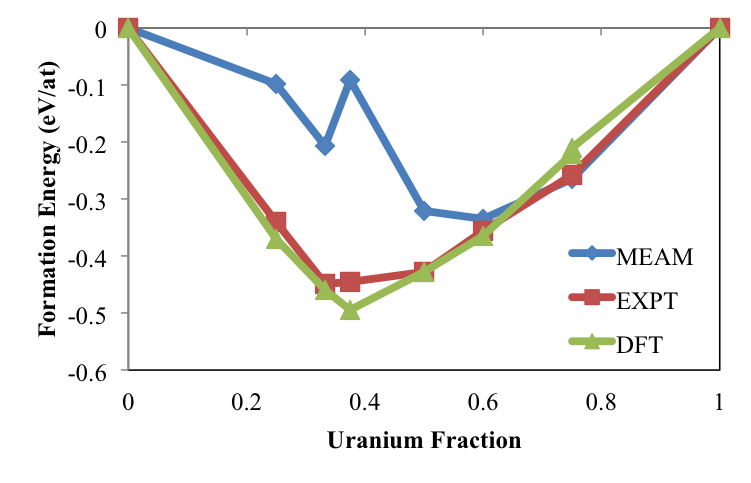
\includegraphics[width=0.8\textwidth]{EvsC_KK1.png}
    \caption{Formation energy per atom as a function of uranium concentration for a variety of phases in the U-Si system as calculated by the MEAM potential and compared to DFT calculations \cite{noordhoek2016} and experiments \cite{berche2009}.}\label{fig:eform3}
\end{figure}

 \begin{figure}[hbt]
	\centering
	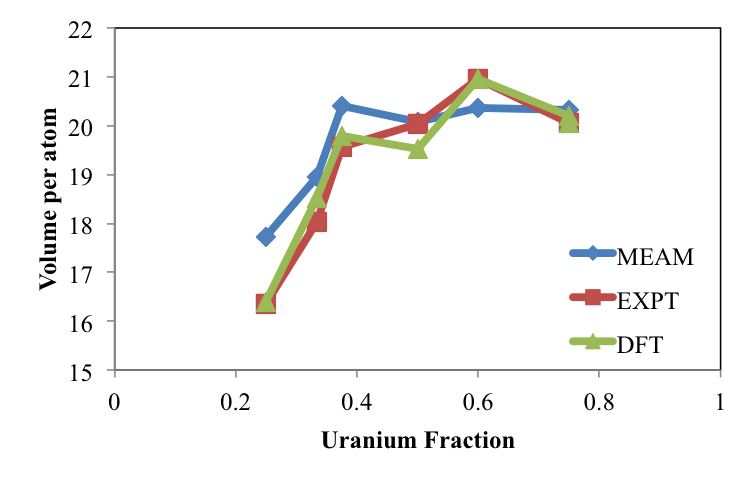
\includegraphics[width=0.8\textwidth]{VvsC_KK1.png}
    \caption{Volume per atom as a function of uranium concentration for a variety of phases in the U-Si system as calculated by the MEAM potential and compared to DFT calculations \cite{noordhoek2016} and experiments \cite{berche2009}.}\label{fig:vol3}
\end{figure}

\FloatBarrier

Although the ability to accurately predict the properties of a variety of crystal structures at 0 K is a critical step in the generation of a reasonable interatomic potential, being able to accurately model systems at non-zero temperatures is necessary to fully utilize the strength of molecular dynamics in branching the atomistic and mesoscopic time and length scales.  Thus, the nature of U$_{3}$Si$_{2}$ was examined as a function of temperature.  A 800 atom (4$\times$4$\times$5 unit cells) supercell is equilibrated at a given temperature in an NPT ensemble utilizing a Nose-Hoover barostat and a Langevin thermostat in the Gr{\o}nbech-Jensen-Farago \cite{gjf2013} formalism with a 1 fs timestep.  The damping parameters for the Nose-Hoover barostat and the Langevin thermostat are 0.1 and 0.01, respectively.  The target pressure is zero with the $\it{x}$, $\it{y}$ and $\it{z}$ components independently controlled. The systems are equilibrated for 100 ps, with energies and volumes determined by averaging over the final 50 ps of the simulation.  The total energy and total volume of the supercell as a function of temperature are displayed in Figure \ref{fig:temp}.  It is observed that the structure is stable and behaves predictably as a function of temperature.   There are no observed crystal structure changes or discontinuities suggesting potential instabilities.  This agrees with experimental observations that find no phase transformations as a function of temperature.  The structure was visually confirmed to be U$_{3}$Si$_{2}$ throughout the temperature range investigated.  The normalized lattice constants are also analyzed as a function of temperature to ensure there exist no structural irregularities.  These are displayed in Figure \ref{fig:latticetemp}.  There is expansion of the $\it{a}$ and $\it{b}$ lattice constants in equal proportion as temperature increases, suggesting the tetragonal symmetry of the crystal structure is retained.  The $\it{c}$ lattice constant also shows a gradual increase as a function of temperature, in a measure slightly greater than that of the $\it{a}$ and $\it{b}$ lattice constants, indicating a slight increase in the $\it{c/a}$ ratio as temperature increases.  

From Figure \ref{fig:temp}, the thermal expansion can be extracted.  The calculated MEAM average linear thermal expansion from 200 K to 1200 K is 11.8$\times$10$^{-6}$ K$^{-1}$ for the U-Si MEAM potential, while the experimental linear thermal expansion is 14-17$\times$10$^{-6}$ K$^{-1}$ from Shimizu \cite{shimizu1965} and 16.1$\times$10$^{-6}$ K$^{-1}$ from White \cite{white2015}.  While slightly underestimated, this is remarkable agreement given that this was not included into the fitting procedure.  

The molar heat capacity, given by equation \ref{eq:cp}, 

\begin{equation}
\label{eq:cp}
C_{P} = \left(\frac{\delta H}{\delta T}\right)_{P}
\end{equation}

was calculated at 400 K for comparison with White, et al. \cite{white2015}.  The calculated value from the MEAM potential is 134.7 J/mol-K.  This quantity compares very favorably to the Dulong-Petit value of 125 J/mol-K and the experimental value of White, et al., which is 150 J/mol-K.  It should be reiterated that this thermo-physical property was not included into the fitting procedure, and thus this is considered excellent agreement to both theory and experiment.  Regretfully, relatively little other experimental data exists for comparison.  

 \begin{figure}[hbt]
	\centering
	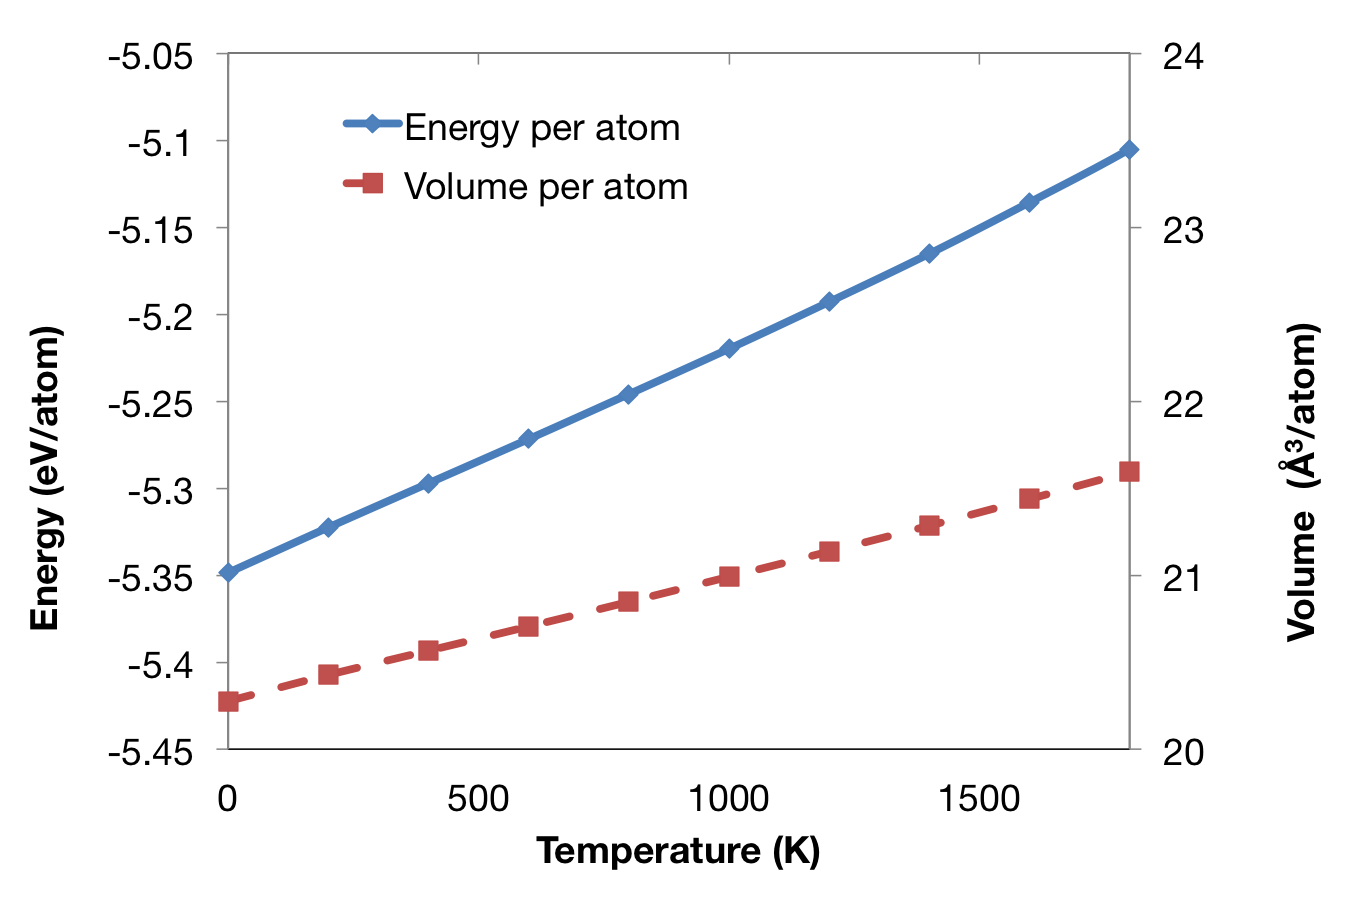
\includegraphics[width=0.8\textwidth]{tempKK1.png}
    \caption{Energy per atom and volume per atom of U$_{3}$Si$_{2}$ as a function of temperature for the U-Si MEAM potential.}\label{fig:temp}
\end{figure}

\begin{figure}[hbt]
	\centering
	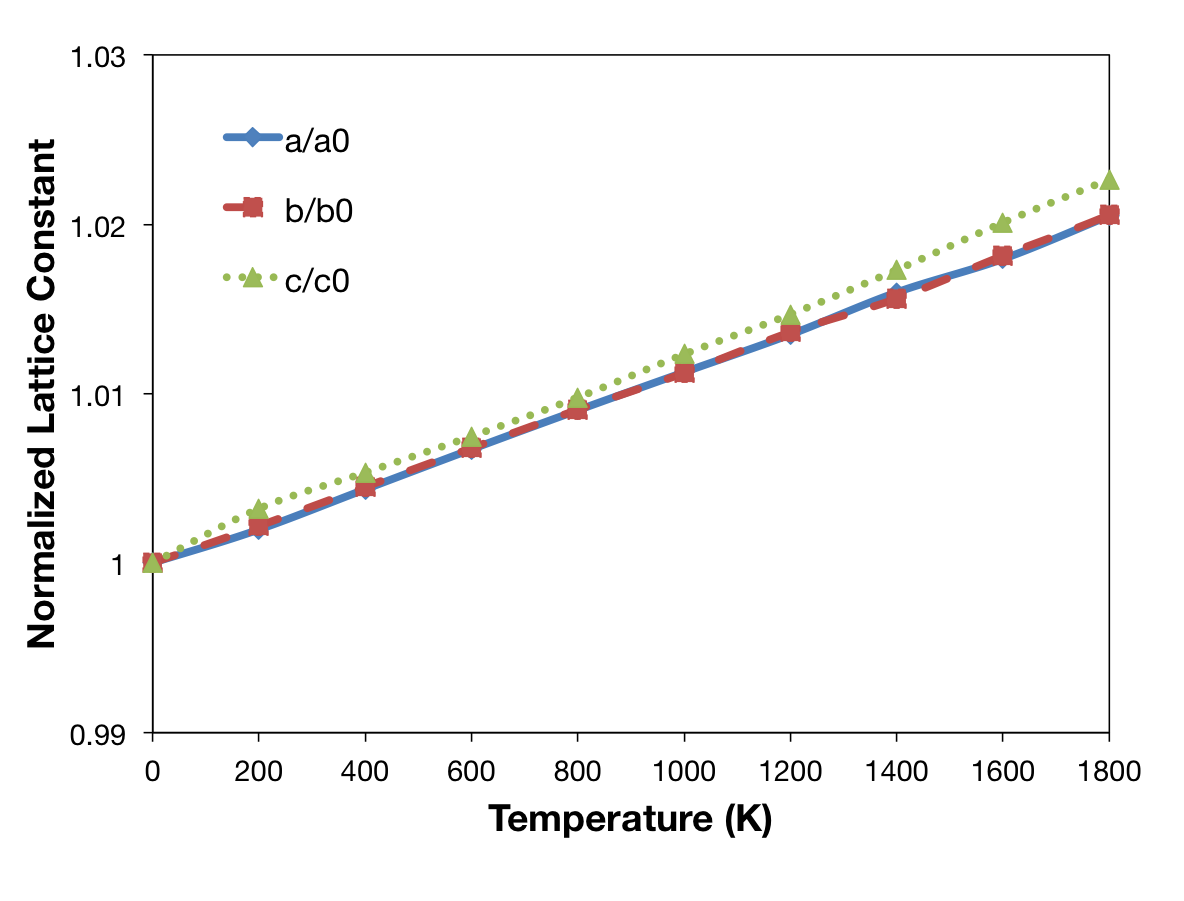
\includegraphics[width=0.8\textwidth]{latticeKK1.png}
    \caption{Variation of normalized lattice constants of U$_{3}$Si$_{2}$ as a function of temperature for the U-Si MEAM potential.}\label{fig:latticetemp}
\end{figure}

\FloatBarrier

The high temperature regime was investigated by calculating the melting point of U$_{3}$Si$_{2}$.  In order to determine the melting point, a two-phase system was constructed consisting of crystal and liquid phases, as in Figure \ref{fig:twophase}.  This system was constructed by holding half of the supercell at a temperature known to be below the melting point and super-heating the other half of the supercell to induce melting.  This system is then evolved at a temperature near the melting point, and the two-phase interface is tracked.  Advancement of the liquid phase into the crystal phase indicates that the system is at a temperature above the melting point.  The system was investigated in increments of 50 K in order to determine a general temperature regime for the melting point of U$_{3}$Si$_{2}$.  The calculated melting point is approximately 1775 K for the U-Si MEAM potential.  The experimental melting point is 1938 K \cite{berche2009}.  Although the melting point is underestimated by approximately 150 K, this is still considered excellent agreement.  

\begin{figure}[hbt]
	\centering
	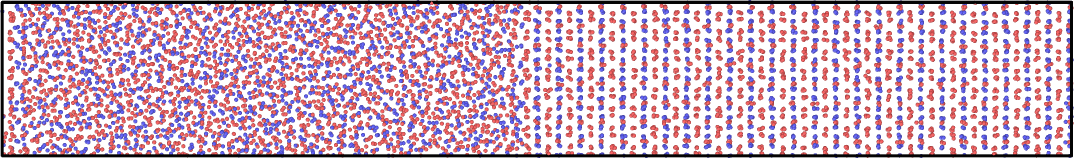
\includegraphics[width=\textwidth]{two_phase2.png}
    \caption{Two-phase system employed in the determination of the melting point of U$_{3}$Si$_{2}$.}\label{fig:twophase}
\end{figure}

\FloatBarrier

As a nuclear fuel, it is necessary that this potential be able to model U$_{3}$Si$_{2}$ under irradiation.  In order to test the ability of the potentials to model radiation damage, a 1 keV cascade is investigated.   The MEAM potentials are splined to a Ziegler-Biersack-Littmark (ZBL) \cite{zbl} potential in the standardized method implemented into LAMMPS.  A 20,000 atom supercell (10$\times$10$\times$20 unit cells) is equilibrated at 500 K for 100 ps in an NPT ensemble with a target pressure of 0 GPa.  In an NVT ensemble, a U1 atom is given additional kinetic energy in the $[$135$]$ direction.  The timestep is reduced to 0.2 fs and the cascade is allowed to evolve for 12 ps.  The residual damage is then evolved at 500 K for 1 ns utilizing a 2 fs timestep.  The state of the cascade and residual damage for the U-Si MEAM potential is displayed in Figure \ref{fig:ben6} at three different times throughout the simulation.  It is observed that the crystal structure is stable and there exists a thermal spike and subsequent annealing stage.  At 0.4 ps after cascade initiation, Wigner-Seitz analysis via Ovito \cite{ovito} shows that there exist 35 Frenkel pairs; there exist 22 Frenkel pairs after 12 ps; there exist 17 Frenkel pairs after 1 ns.  By investigating defects on each species sublattice, it can be determined the general nature of the defects generated via this specific cascade.  Looking strictly at the uranium sublattice after 1 ns, there are 16 Frenkel pairs.  Looking strictly at the silicon sublattice, there are 12 Frenkel pairs.  This gives a total of 28 defects.  It can thus be determined that in the total system there exist 17 Frenkel pairs and 8 anti-site defects after 1 ns, with approximately the same number of defects on each sublattice.  It can be concluded that this potential is displaying reasonable behavior under irradiation and the nature and number of defects can be readily determined.  It should be noted that this is not intended to be a full radiation damage study, but simply an example that this potential produces reasonable radiation damage behavior.  Radiation damage studies are certainly warranted in the future.  

\begin{figure}[bt]
	\centering
	\includegraphics[width=\textwidth]{KK_cascadetotalb.png}
    \caption{1 keV cascade behavior of U$_{3}$Si$_{2}$ at 500 K.  The left-most panel is 0.4 ps after cascade initiation; the middle panel is 12 ps after cascade initiation; the right-most panel is 1 ns after cascade initiation.}\label{fig:ben6}
\end{figure}

\FloatBarrier

Another microstructural feature of interest is free surfaces.  To investigate the nature of free surfaces, two systems are created to investigate both the (100) free surface and the (001) free surface (there exist multiple possible terminations, but in this work all terminuses are created at unit cell boundaries).  For the (100) free surface, a system supercell of 30$\times$6$\times$8 unit cells (14400 atoms) was generated.  A vacuum region was created by increasing the simulation domain by 10$\%$ in the $\it{x}$ direction.  For the (001) free surface, a system supercell of 5$\times$5$\times$40 unit cells (10000 atoms) was generated.  A vacuum region was created by increasing the simulation domain by 10$\%$ in the $\it{z}$ direction.  This methodology creates two unique surfaces and thus the reported surface energy is an average between the two surfaces.  This methodology also ensures that stoichiometry is maintained and the system can be directly compared to pure U$_{3}$Si$_{2}$.  Both longer and shorter systems were analyzed with more vacuum region and it was determined that this setup provided an accurate determination of the surface energies.  The system with free surfaces is equilibrated in an NPT ensemble at 500 K for 100 ps and the average energy is determined over the final 50 ps of the simulation.  The relaxed structures of the (100) and (001) free surfaces are shown in Figure \ref{fig:ben7} and Figure \ref{fig:ben8}, respectively.  The first thing to notice is that the bulk structure remains stable and retains its crystal symmetry.  The surface energies are determined by equation \ref{eq:surface}

\begin{equation}
\label{eq:surface}
E_{surf}= \frac{(E^{*} - E)}{SA} * N
\end{equation}

where $\it{E^{*}}$ is the energy per atom of the system with two free surfaces, $\it{E}$ is the energy per atom of the perfect crystal U$_{3}$Si$_{2}$, $\it{SA}$ is the total free surface area (two free surfaces are present in the system) and $\textit{N}$ is the number of atoms in the system with two free surfaces.  The resultant energy for the (100) surface is 1.73 J/m$^{2}$ and the (001) surface energy is 1.75 J/m$^{2}$.  A prior DFT study investigated free surfaces in U$_{3}$Si$_{2}$ \cite{anl_report, miao2017}.  The surface energy was found to vary from 1.16 J/m$^{2}$ to 1.48 J/m$^{2}$.  In this DFT study, the (100) surface had a surface energy of 1.48 J/m$^{2}$, while the (001) surface had a surface energy of 1.43 J/m$^{2}$.  The nature of the lowest energy surface was not reported, but an average surface energy was estimated at 1.32 J/m$^{2}$.  Thus, the surface energy predicted from the MEAM potential is slightly higher than that from DFT calculations, but still in reasonable agreement.  Given that the physical nature of the surfaces as predicted by the MEAM potentials is reasonable combined with the calculation of reasonable surface energies, it is suggested that the interatomic potential performs adequately for free surfaces in U$_{3}$Si$_{2}$.  

\begin{figure}[bt]
	\centering
	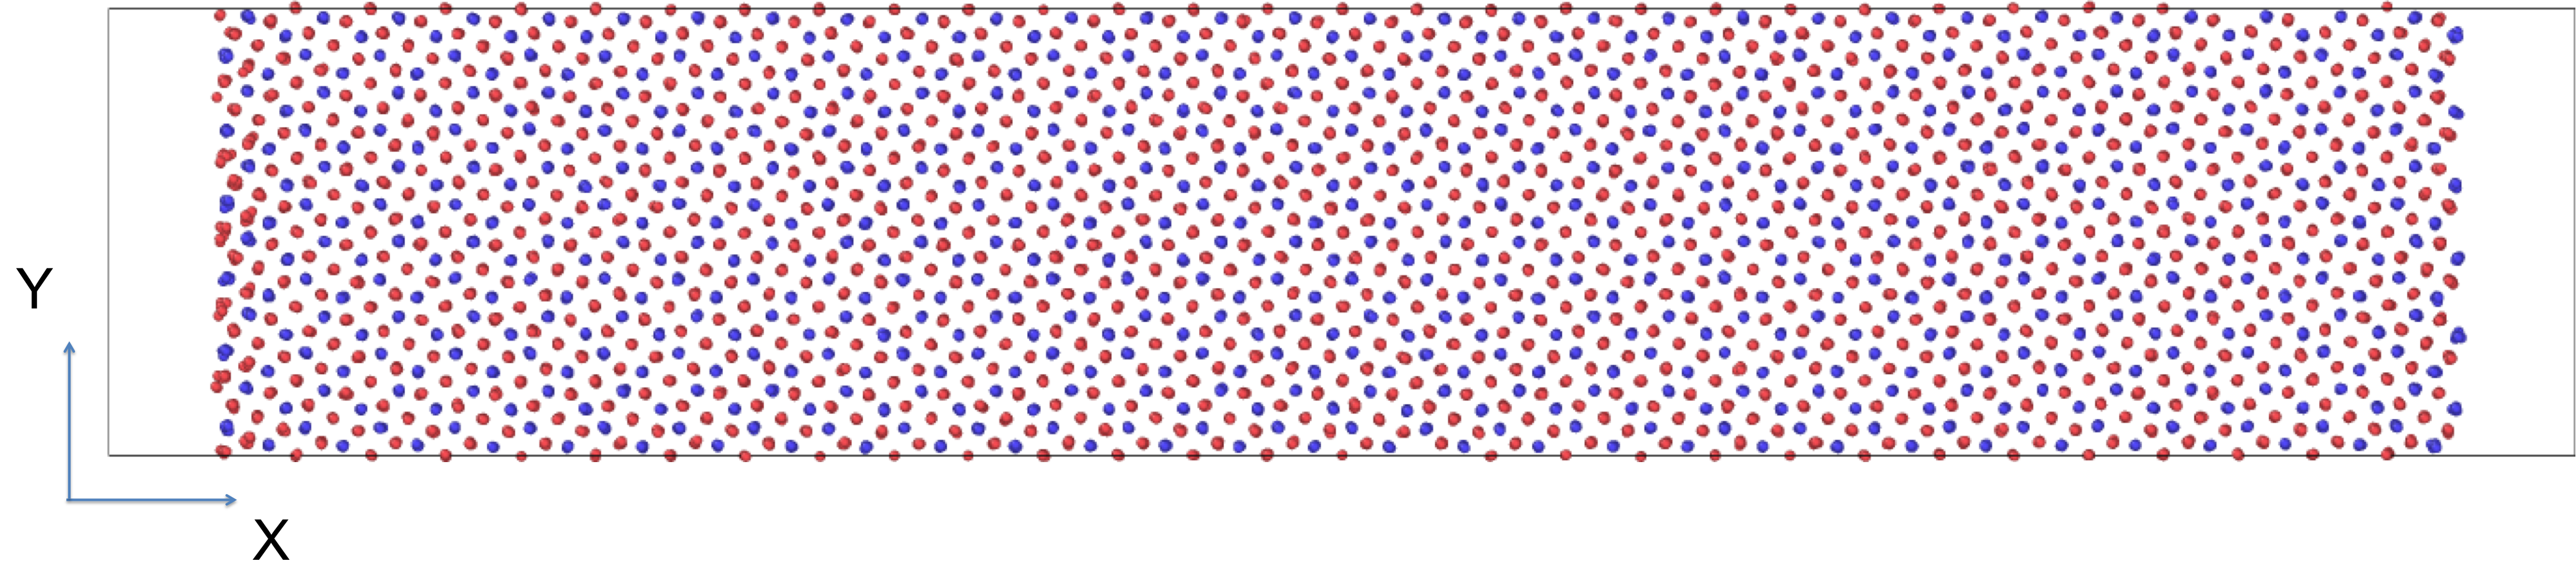
\includegraphics[width=0.9\textwidth]{100KK1a.png}
    \caption{(100) free surface of U$_{3}$Si$_{2}$ at 500 K after a 100 ps relaxation.}\label{fig:ben7}
\end{figure}

\begin{figure}[bt]
	\centering
	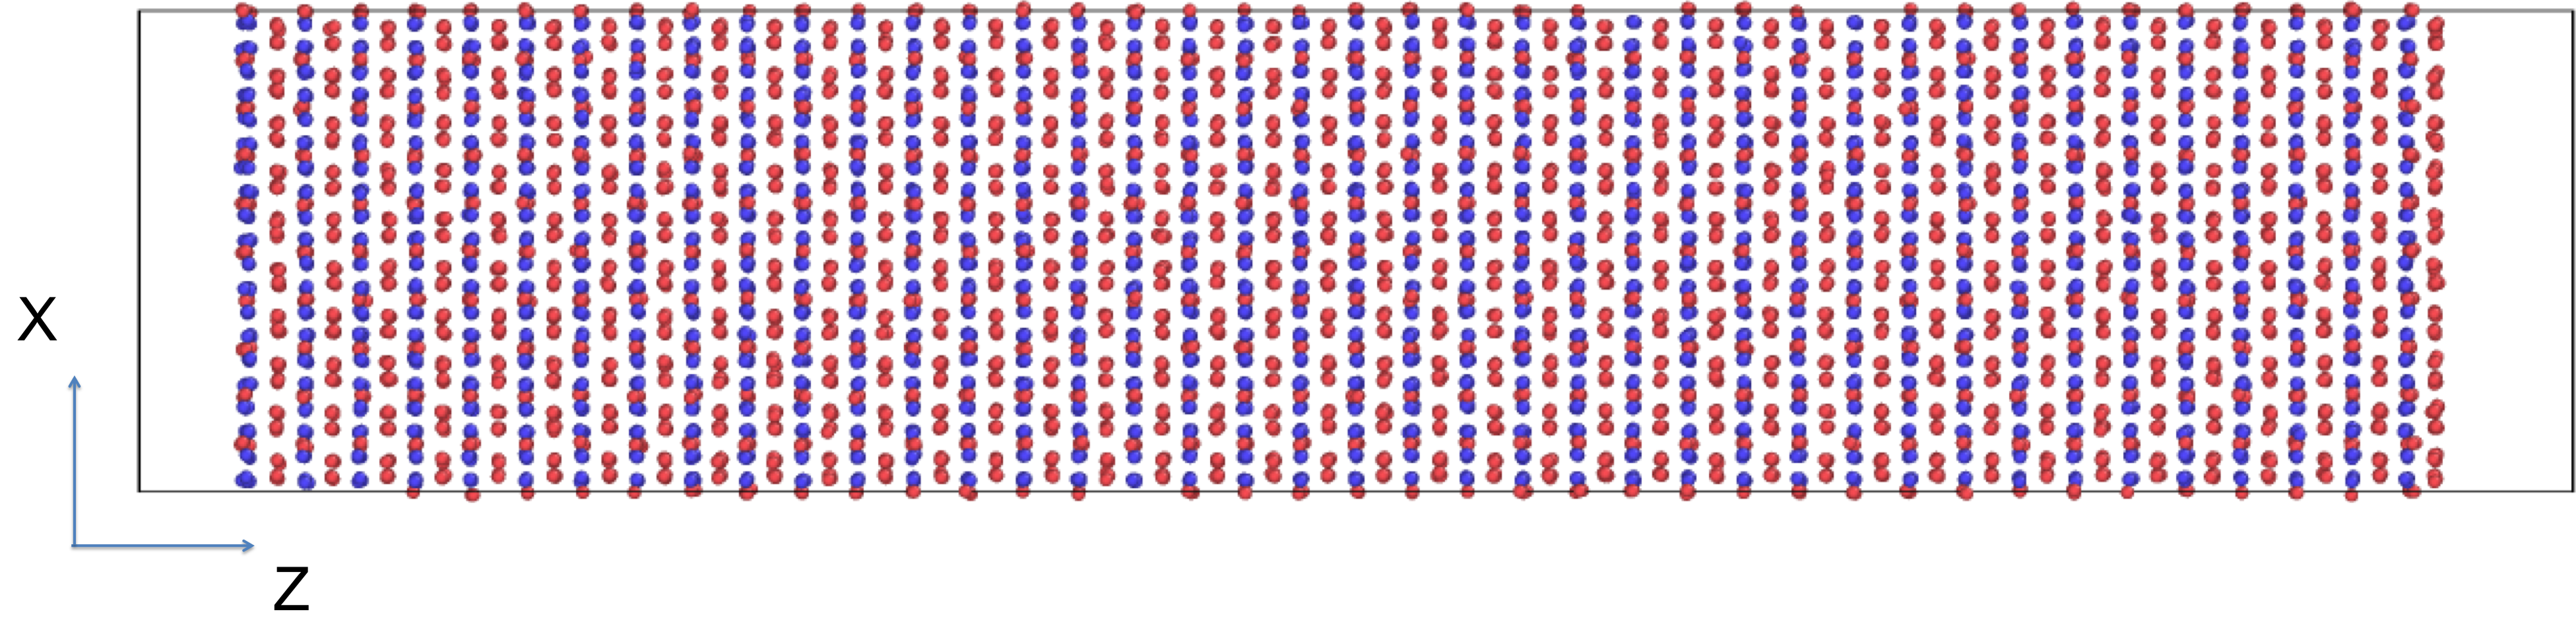
\includegraphics[width=0.9\textwidth]{001KK1a.png}
    \caption{(001) free surface of U$_{3}$Si$_{2}$ at 500 K after a 100 ps relaxation. }\label{fig:ben8}
\end{figure}

\FloatBarrier

To further investigate the performance of the potential, as well as to calculate an average surface energy, a void is introduced into an equilibrated U$_{3}$Si$_{2}$ system, and then further relaxed.  The system with a void is equilibrated in an NPT ensemble at 500 K for 100 ps and the average energy is determined over the final 50 ps of the simulation.  It is observed that voids from a radius of 4 {\AA} up to 32 {\AA} are stable within U$_{3}$Si$_{2}$ up to 100 ps (when simulations were terminated, voids larger than 32 {\AA} were not investigated).   The stoichiometry of the system is ensured to be within 0.001$\%$ of the ideal U$_{3}$Si$_{2}$ system.  A representative void with a radius of 25 {\AA} is shown in Figure \ref{fig:void}.  No void collapse is observed, no crystal structure collapse or distortion is observed, but minimal void surface reconstruction does occur.  This further reinforces the suitability and stability of the potential for non-equilibrium systems.  The void surface energy is determined via equation \ref{eq:surface}, where $\it{SA}$ is the surface area of the void.  The void size is increased, along with system size, until the void surface energy converged.  The representative void surface energy is 1.69 J/m$^{2}$ for the U-Si MEAM potential.

\begin{figure}[bt]
	\centering
	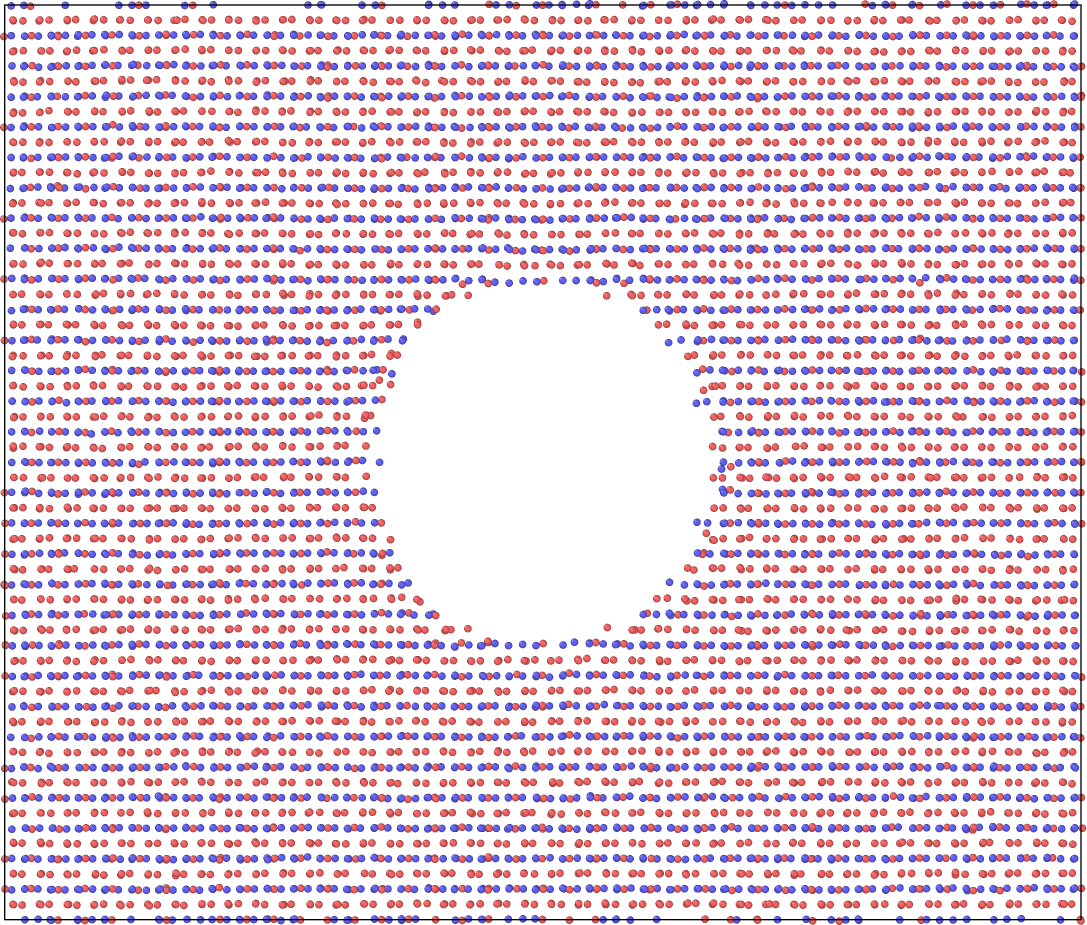
\includegraphics[width=0.8\textwidth]{void3.png}
    \caption{2D projection of a 3D slice through the a U$_{3}$Si$_{2}$ supercell at 500 K containing a void with a radius of 25 {\AA}.  }\label{fig:void}
\end{figure}

\FloatBarrier
\clearpage

\section{Discussion}

The above assessment shows the potential performs satisfactorily for the U$_{3}$Si$_{2}$ phase, but with specific strengths and weaknesses.  The U-Si MEAM potential is sufficiently accurate with regards to cohesive energy and volume per atom at 0 K.  The majority of the defect properties are also accurately reproduced as compared to DFT.  The potential shows excellent behavior in the high temperature regime, with reasonably accurate predictions of the thermal expansion, heat capacity and melting point.  This potential accurately describes the volumes of various U-Si phases across the composition regime, but only accurately describes the formation energies in the U-rich region.  Given that nuclear fuel will operate in the U-rich composition regime, this is only a minor drawback.  

This potential is somewhat weak regarding elastic constants, where it is generally over-stiff and yields a root mean square error of 55 GPa for the reported elastic constants.  The bulk modulus is overestimated by approximately 50 GPa, but the shear modulus is in quite good agreement with DFT results.  Also, although the majority of defect formation energies are accurately reproduced, there is a significant enough variance from DFT for the U1 vacancy and the Si antisite defect that care should be taken in systems where these defects are prevalent.  Finally, this potential is not intended for investigation of liquid phase U$_{3}$Si$_{2}$.  Although the potential performs very well for melting point of U$_{3}$Si$_{2}$, further validation should be conducted before undertaking work focused on the liquid phase. 

Given the complex nature of the crystal structure of U$_{3}$Si$_{2}$, the inherent difficulties associated with the development of atomic potentials for pure uranium, let alone uranium-alloys, it is the opinion of the authors that a suitable interatomic potential to describe the U-Si system has been developed.  Provided that the scientific community is continually gaining more knowledge on U-Si alloys via experimentation and first principles examinations, future refinement of the potentials should be undertaken once more atomistic and fundamental property information has been gathered.  

\section{Conclusion}

A modified Embedded-Atom Method interatomic potential was developed for the U-Si system.  The potential accurately describe 0 K properties of the primary phase of interest (U$_{3}$Si$_{2}$), including formation energy, lattice constants and several point defect properties.  The potential can also reasonably predict properties of a range of U-Si phases across the composition spectrum.  The predicted thermal expansion, heat capacity and melting point compare favorably to reported experimental values.  The interatomic potential was tested by investigating the behavior of U$_{3}$Si$_{2}$ under a 1 keV cascade, with free surfaces and in the presence of a void.  The potential behaves in a reasonable manner in each of these three non-equilibrium cases.  This potential can serve as a tool to branch experiments and recent first principles calculations to longer time and larger length scale simulations.

\section{Acknowledgments}
This work is supported by the U.S. Department of Energy, Office of Nuclear Energy, Nuclear Energy Advanced Modeling and Simulation (NEAMS) Accident Tolerant Fuel High-Impact-Problem Program. This manuscript has been authored by Battelle Energy Alliance, LLC under Contract No. DEAC07-05ID14517 with the U.S. Department of Energy. The United States Government retains and the publisher, by accepting the article for publication, acknowledges that the United States Government retains a nonexclusive, paid-up, irrevocable, world-wide license to publish or reproduce the published form of this manuscript, or allow others to do so, for United States Government purposes.  Los Alamos National Laboratory, an affirmative action/equal opportunity employer, is operated by Los Alamos National Security, LLC, for the National Nuclear Security Administration of the U.S. Department of Energy under Contract No. DE-AC52-06NA25396.  This research made use of the resources of the High Performance Computing Center at Idaho National Laboratory, which is supported by the Office of Nuclear Energy of the U.S. Department of Energy and the Nuclear Science User Facilities under Contract No. DE-AC07-05ID14517.

\begin{comment}
\begin{appendix}
\section{Calculation of point defect energies in U$_{3}$Si$_{2}$}
Consider a base alloy A$_{x0}$B$_{1-x0}$ and energy per atom e$_{0}$ and a second phase with concentration of A$_{x\phi}$B$_{1-x\phi}$ and energy per atom e$_{\phi}$.  The energy per atom e$_{2phase}$ as function of composition is given by:

\begin{equation}
\label{eq:def1}
e_{2phase}(x)=\frac{x-x_{0}}{x_{\phi}-x_{0}}e_{\phi} + \frac{x_{\phi}-x}{x_{\phi}-x_{0}}e_{0} 
\end{equation}

Consider an A defect in the base alloy that changes stoichiometry, e.g., vacancy (V) (remove A atom), interstitial (I) (add A atom), or anti-site defect (AS) (add A atom and remove B atom).  We are interested in the energetics of a dilute solution of defects, but can conveniently calculate defect energies in only small 3D periodic systems.  Consider a small system with N atoms of base alloy with one defect and supercell energy E$_{d}$.  The number of atoms in this cell, N$_{d}$, is given by:

\begin{equation}
\label{eq:def2}
N_{d} = N + i_{d}
\end{equation}

where i$_{d}$ is the change in atoms with defect, e.g., i$_{d}$=1,0,-1 for the interstitial, anti-site defect, and vacancy respectively.  The number of A atoms in this cell, N$_{dA}$, is given by:

\begin{equation}
\label{eq:def3}
N_{dA} = x_{0}N + A_{d}
\end{equation}

where 

\begin{equation}
\label{eq:def4}
A_{d} = \begin{cases}
    1       & \quad d = I \\
    1       & \quad d = AS\\
    -1      & \quad d = V\\
  \end{cases} 
\end{equation}

The concentration in the cell x$_{d}$ is given by:

\begin{equation}
\label{eq:def5}
x_{d}=\frac{N_{dA}}{N_{d}} 
\end{equation}

The defect formation energy per cell may be defined as

\begin{equation}
\label{eq:def6}
E_{defect} = E_{d} - N_{d}e_{2phase}(x_{d})
\end{equation}

A convenient way to compare energies is to use atomic energies. We can express the energy of the 2-phase system as

\begin{equation}
\label{eq:def7}
e_{2phase}(x_{A}) = e_{A}x_{A} + e_{B}(1-x_{A})
\end{equation}

It is convenient to determine E$_{A}$ and E$_{B}$ by using the energies of the two phases.

\begin{equation}
\label{eq:def8}
e_{0} = e_{A}x_{0} + e_{B}(1-x_{0})
\end{equation}	 

\begin{equation}
\label{eq:def9}
e_{\phi} = e_{A}x_{\phi} + e_{B}(1-x_{\phi})
\end{equation}

which results in

\begin{equation}
\label{eq:def10}
e_{A}=\frac{e_{0}(1-x_{\phi})-e_{\phi}(1-x_{0})}{x_{0}-x_{\phi}} 
\end{equation}

\begin{equation}
\label{eq:def11}
e_{B}=\frac{e_{0}x_{\phi}-e_{\phi}x_{0}}{x_{\phi}-x_{0}} 
\end{equation}

So the defect formation energy is

\begin{equation}
\label{eq:def12}
E_{defect} = E_{d} - N_{d}[e_{A}x_{d} + e_{B}(1-x_{d})] = E_{d} - Ne_{0} - e_{A}A_{d} - e_{B}(i_{d}-A_{d})
\end{equation}

It should be noted that the two reference phases utilized in the determination of defect energies are $\alpha$-U$_{3}$Si and FeB-USi.

\end{appendix}
\end{comment}

\bibliography{MARMOTbib.bib}

\end{document}




